\section{Symbol Variants}

\begin{frame}{\secname}
  \textbf{Problem}
  \begin{itemize}
    \item Impossible to have different symbols for the same component\\
          e.g. Resistor: 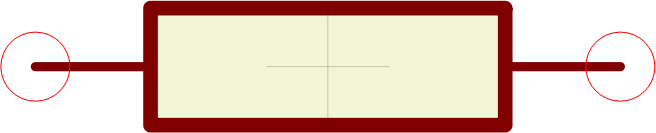
\includegraphics[height=4mm]{images/R-EU_symbol.png}
          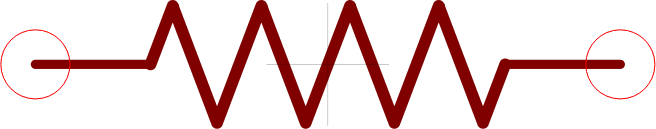
\includegraphics[height=4mm]{images/R-US_symbol.png}
  \end{itemize}

  \pause

  \textbf{Result}
  \begin{itemize}
    \item Duplicate components (same functionality, different symbol)
  \end{itemize}
\end{frame}

\begin{frame}[fragile]{\secname}
  \vspace*{-2\baselineskip}\leavevmode % reduce space
  \begin{center}
    \begin{tikzpicture}
    \matrix (m) [row sep={7mm,between origins}, column sep={.26\textwidth,between origins}] {
      \onslide<1->{\node (tcmp) [anchor=center] {\textbf{Device}};} &
      \onslide<1->{\node (tcmp) [anchor=center] {\textbf{Component}};} &
      \onslide<6->{\node (tvar) [anchor=center] {\textbf{Variant}};} &
      \onslide<1->{\node (tsym) [anchor=center] {\textbf{Symbol}};} \\

      % rows 1-3
      \node (dev11) [lpbox, text width=15mm, anchor=center] {
        \textbf{R-0603}
      }; & & & \\
      \node (dev12) [lpbox, text width=15mm, anchor=center] {
        \textbf{R-0805}
      }; &
      \node (cmp1) [lpbox, text width=15mm, anchor=center] {
        \textbf{\only<1-2,6->{R}\only<3-5>{R-EU}}
      }; &
      \onslide<6->{\node (var1) [lpbox, text width=15mm, anchor=center] {
        \textbf{EU}
      };} &
      \node (sym1) [anchor=center] {
        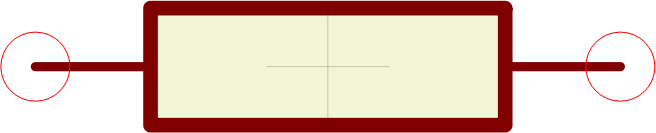
\includegraphics[height=5mm]{images/R-EU_symbol.png}
      }; \\
      \node (dev13) [lpbox, text width=15mm, anchor=center] {
        \textbf{R-1206}
      }; & & & \\

      % rows 4-6
      \onslide<4-5>{\node (dev21) [lpbox, text width=15mm, anchor=center] {
        \textbf{R-0603}
      };} & & & \\
      \onslide<4-5>{\node (dev22) [lpbox, text width=15mm, anchor=center] {
        \textbf{R-0805}
      };} &
      \onslide<3-5>{\node (cmp2) [lpbox, text width=15mm, anchor=center] {
        \textbf{R-US}
      };} &
      \onslide<6->{\node (var2) [lpbox, text width=15mm, anchor=center] {
        \textbf{US}
      };} &
      \onslide<2->{\node (sym2) [anchor=center] {
        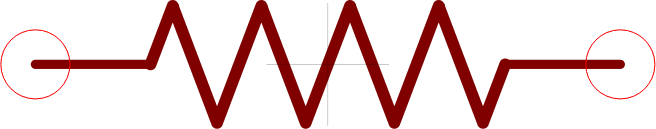
\includegraphics[height=5mm]{images/R-US_symbol.png}
      };} \\
      \onslide<4-5>{\node (dev23) [lpbox, text width=15mm, anchor=center] {
        \textbf{R-1206}
      };} & & & \\

      % rows 7-9
      \onslide<5-5>{\node (dev31) [lpbox, text width=15mm, anchor=center] {
        \textbf{R-0603}
      };} & & & \\
      \onslide<5-5>{\node (dev32) [lpbox, text width=15mm, anchor=center] {
        \textbf{R-0805}
      };} &
      \onslide<5-5>{\node (cmp3) [lpbox, text width=15mm, anchor=center] {
        \textbf{R-small}
      };} &
      \onslide<6->{\node (var3) [lpbox, text width=15mm, anchor=center] {
        \textbf{small}
      };} &
      \onslide<5->{\node (sym3) [anchor=center] {
        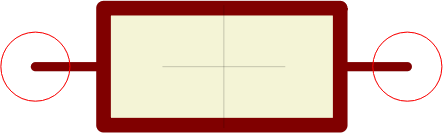
\includegraphics[height=5mm]{images/R-small_symbol.png}
      };} \\
      \onslide<5-5>{\node (dev33) [lpbox, text width=15mm, anchor=center] {
        \textbf{R-1206}
      };} & & & \\
    };

    % box
    \begin{pgfonlayer}{background}
    \onslide<6->{
      \node[fill=yellow!60, fit=(tvar)(var3), inner sep=3mm, rounded corners] {};
    }
    \end{pgfonlayer}

    % lines
    \begin{pgfonlayer}{background}
      % device -> component
      \draw<1->[lpline, draw=red, ultra thick] (dev11.east) -- (cmp1.west);
      \draw<1->[lpline, draw=red, ultra thick] (dev12.east) -- (cmp1.west);
      \draw<1->[lpline, draw=red, ultra thick] (dev13.east) -- (cmp1.west);
      \draw<4-5>[lpline, draw=red, ultra thick] (dev21.east) -- (cmp2.west);
      \draw<4-5>[lpline, draw=red, ultra thick] (dev22.east) -- (cmp2.west);
      \draw<4-5>[lpline, draw=red, ultra thick] (dev23.east) -- (cmp2.west);
      \draw<5-5>[lpline, draw=red, ultra thick] (dev31.east) -- (cmp3.west);
      \draw<5-5>[lpline, draw=red, ultra thick] (dev32.east) -- (cmp3.west);
      \draw<5-5>[lpline, draw=red, ultra thick] (dev33.east) -- (cmp3.west);
  
      % component -> symbol
      \draw<1-5>[lpline, draw=red, ultra thick] (cmp1.east) -- (sym1.west);
      \draw<3-5>[lpline, draw=red, ultra thick] (cmp2.east) -- (sym2.west);
      \draw<5-5>[lpline, draw=red, ultra thick] (cmp3.east) -- (sym3.west);
  
      % component -> variant
      \draw<6->[lpline, draw=red, ultra thick] (cmp1.east) -- (var1.west);
      \draw<6->[lpline, draw=red, ultra thick] (cmp1.east) -- (var2.west);
      \draw<6->[lpline, draw=red, ultra thick] (cmp1.east) -- (var3.west);
  
      % variant -> symbol
      \draw<6->[lpline, draw=red, ultra thick] (var1.east) -- (sym1.west);
      \draw<6->[lpline, draw=red, ultra thick] (var2.east) -- (sym2.west);
      \draw<6->[lpline, draw=red, ultra thick] (var3.east) -- (sym3.west);
    \end{pgfonlayer}
    \end{tikzpicture}
  \end{center}
\end{frame}
